\documentclass[10pt,A4]{article}
\usepackage[top=0.85in,left=2.75in,footskip=0.75in]{geometry}

% Use adjustwidth environment to exceed column width (see example table in text)
\usepackage{changepage}

% Use Unicode characters when possible
\usepackage[utf8]{inputenc}
\usepackage{booktabs,caption,fixltx2e}
\usepackage[flushleft]{threeparttable}
\usepackage{tabularx}
% textcomp package and marvosym package for additional characters
\usepackage{textcomp,marvosym}

% fixltx2e package for \textsubscript
\usepackage{fixltx2e}

% amsmath and amssymb packages, useful for mathematical formulas and symbols
\usepackage{amsmath,amssymb}

% cite package, to clean up citations in the main text. Do not remove.
\usepackage{cite}

% Use nameref to cite supporting information files (see Supporting Information section for more info)
\usepackage{nameref,hyperref}

% line numbers
\usepackage[right]{lineno}

% ligatures disabled
\usepackage{microtype}
%\DisableLigatures[f]{encoding = *, family = * }

% rotating package for sideways tables
\usepackage{rotating}

% Remove comment for double spacing
\usepackage{setspace} 
\doublespacing

% Text layout
\raggedright
\setlength{\parindent}{0.5cm}
\textwidth 5.25in 
\textheight 8.75in

% Bold the 'Figure #' in the caption and separate it from the title/caption with a period
% Captions will be left justified
\usepackage[aboveskip=1pt,labelfont=bf,labelsep=period,justification=raggedright,singlelinecheck=off]{caption}

% Use the PLoS provided BiBTeX style
\bibliographystyle{plos2015}

% Remove brackets from numbering in List of References
\makeatletter
\renewcommand{\@biblabel}[1]{\quad#1.}
\makeatother

% Leave date blank
\date{}

% Header and Footer with logo
\usepackage{lastpage,fancyhdr,graphicx}
\usepackage{ragged2e}

\usepackage{color}
\usepackage[dvipsnames]{xcolor}

%\usepackage{epstopdf}
\pagestyle{myheadings}
\pagestyle{fancy}
\fancyhf{}
\lhead{

\includegraphics[width=1.6in]{figures/pone.png}
}
\rhead{Classifying Patents Based on their Semantic Content\vspace{2mm}}
\rfoot{\thepage}
\renewcommand{\footrule}{\hrule height 2pt \vspace{2mm}}
\fancyheadoffset[L]{2.25in}
\fancyfootoffset[L]{2.25in}
\lfoot{\sf Bergeaud, Potiron and Raimbault, 2017}
%\lfoot{}

%% Include all macros below

\newcommand{\lorem}{{\bf LOREM}}
\newcommand{\ipsum}{{\bf IPSUM}}

%%%%%%%%%%%%%%%%%%%%%%
%% User-defined commands
%%%%%%%%%%%%%%%%%%%%%%


%Yoann's commands
\newcommand{\reels}{\mathbb{R}}
\newcommand{\naturels}{\mathbb{N}}
\newcommand{\relatifs}{\mathbb{Z}}
\newcommand{\rat}{\mathbb{Q}}
\newcommand{\complex}{\mathbb{C}}
\newcommand{\esp}{\mathbb{E}}
\newcommand{\proba}{\mathbb{P}}
\newcommand{\var}{\operatorname{Var}}
\newcommand{\cov}{\operatorname{Cov}}
\newcommand{\Tau}{\mathrm{T}}



% writing utilities

% comments and responses
\usepackage{xparse}
\DeclareDocumentCommand{\comment}{m o o o o}
{%
    \textcolor{red}{#1}
    \IfValueT{#2}{\textcolor{blue}{#2}}
    \IfValueT{#3}{\textcolor{ForestGreen}{#3}}
    \IfValueT{#4}{\textcolor{red!50!blue}{#4}}
    \IfValueT{#5}{\textcolor{Aquamarine}{#5}}
}


% todo
\newcommand{\todo}[1]{\textcolor{red!50!blue}{\textbf{\textit{#1}}}}




%% END MACROS SECTION


\begin{document}
\vspace*{0.35in}


\justify









%\end{document}





\section*{S4 Text : Network Sensitivity Analysis \label{app:sensitivity}}


\subsubsection*{Network Sensitivity}

The example of Fig.1 in main text for a given year yielded the same qualitative behavior for all years, as shown in Fig.~\ref{fig:ext-sensitivity-1}, \ref{fig:ext-sensitivity-2} and \ref{fig:ext-sensitivity-3} here.  We also show an other point of view over the Pareto optimization, that is the third plot giving the values of normalized objectives as a function of $\theta_c$.

% Figures :

%%%%%%%%%%%%%%%%%%%%
\begin{figure}
\centering
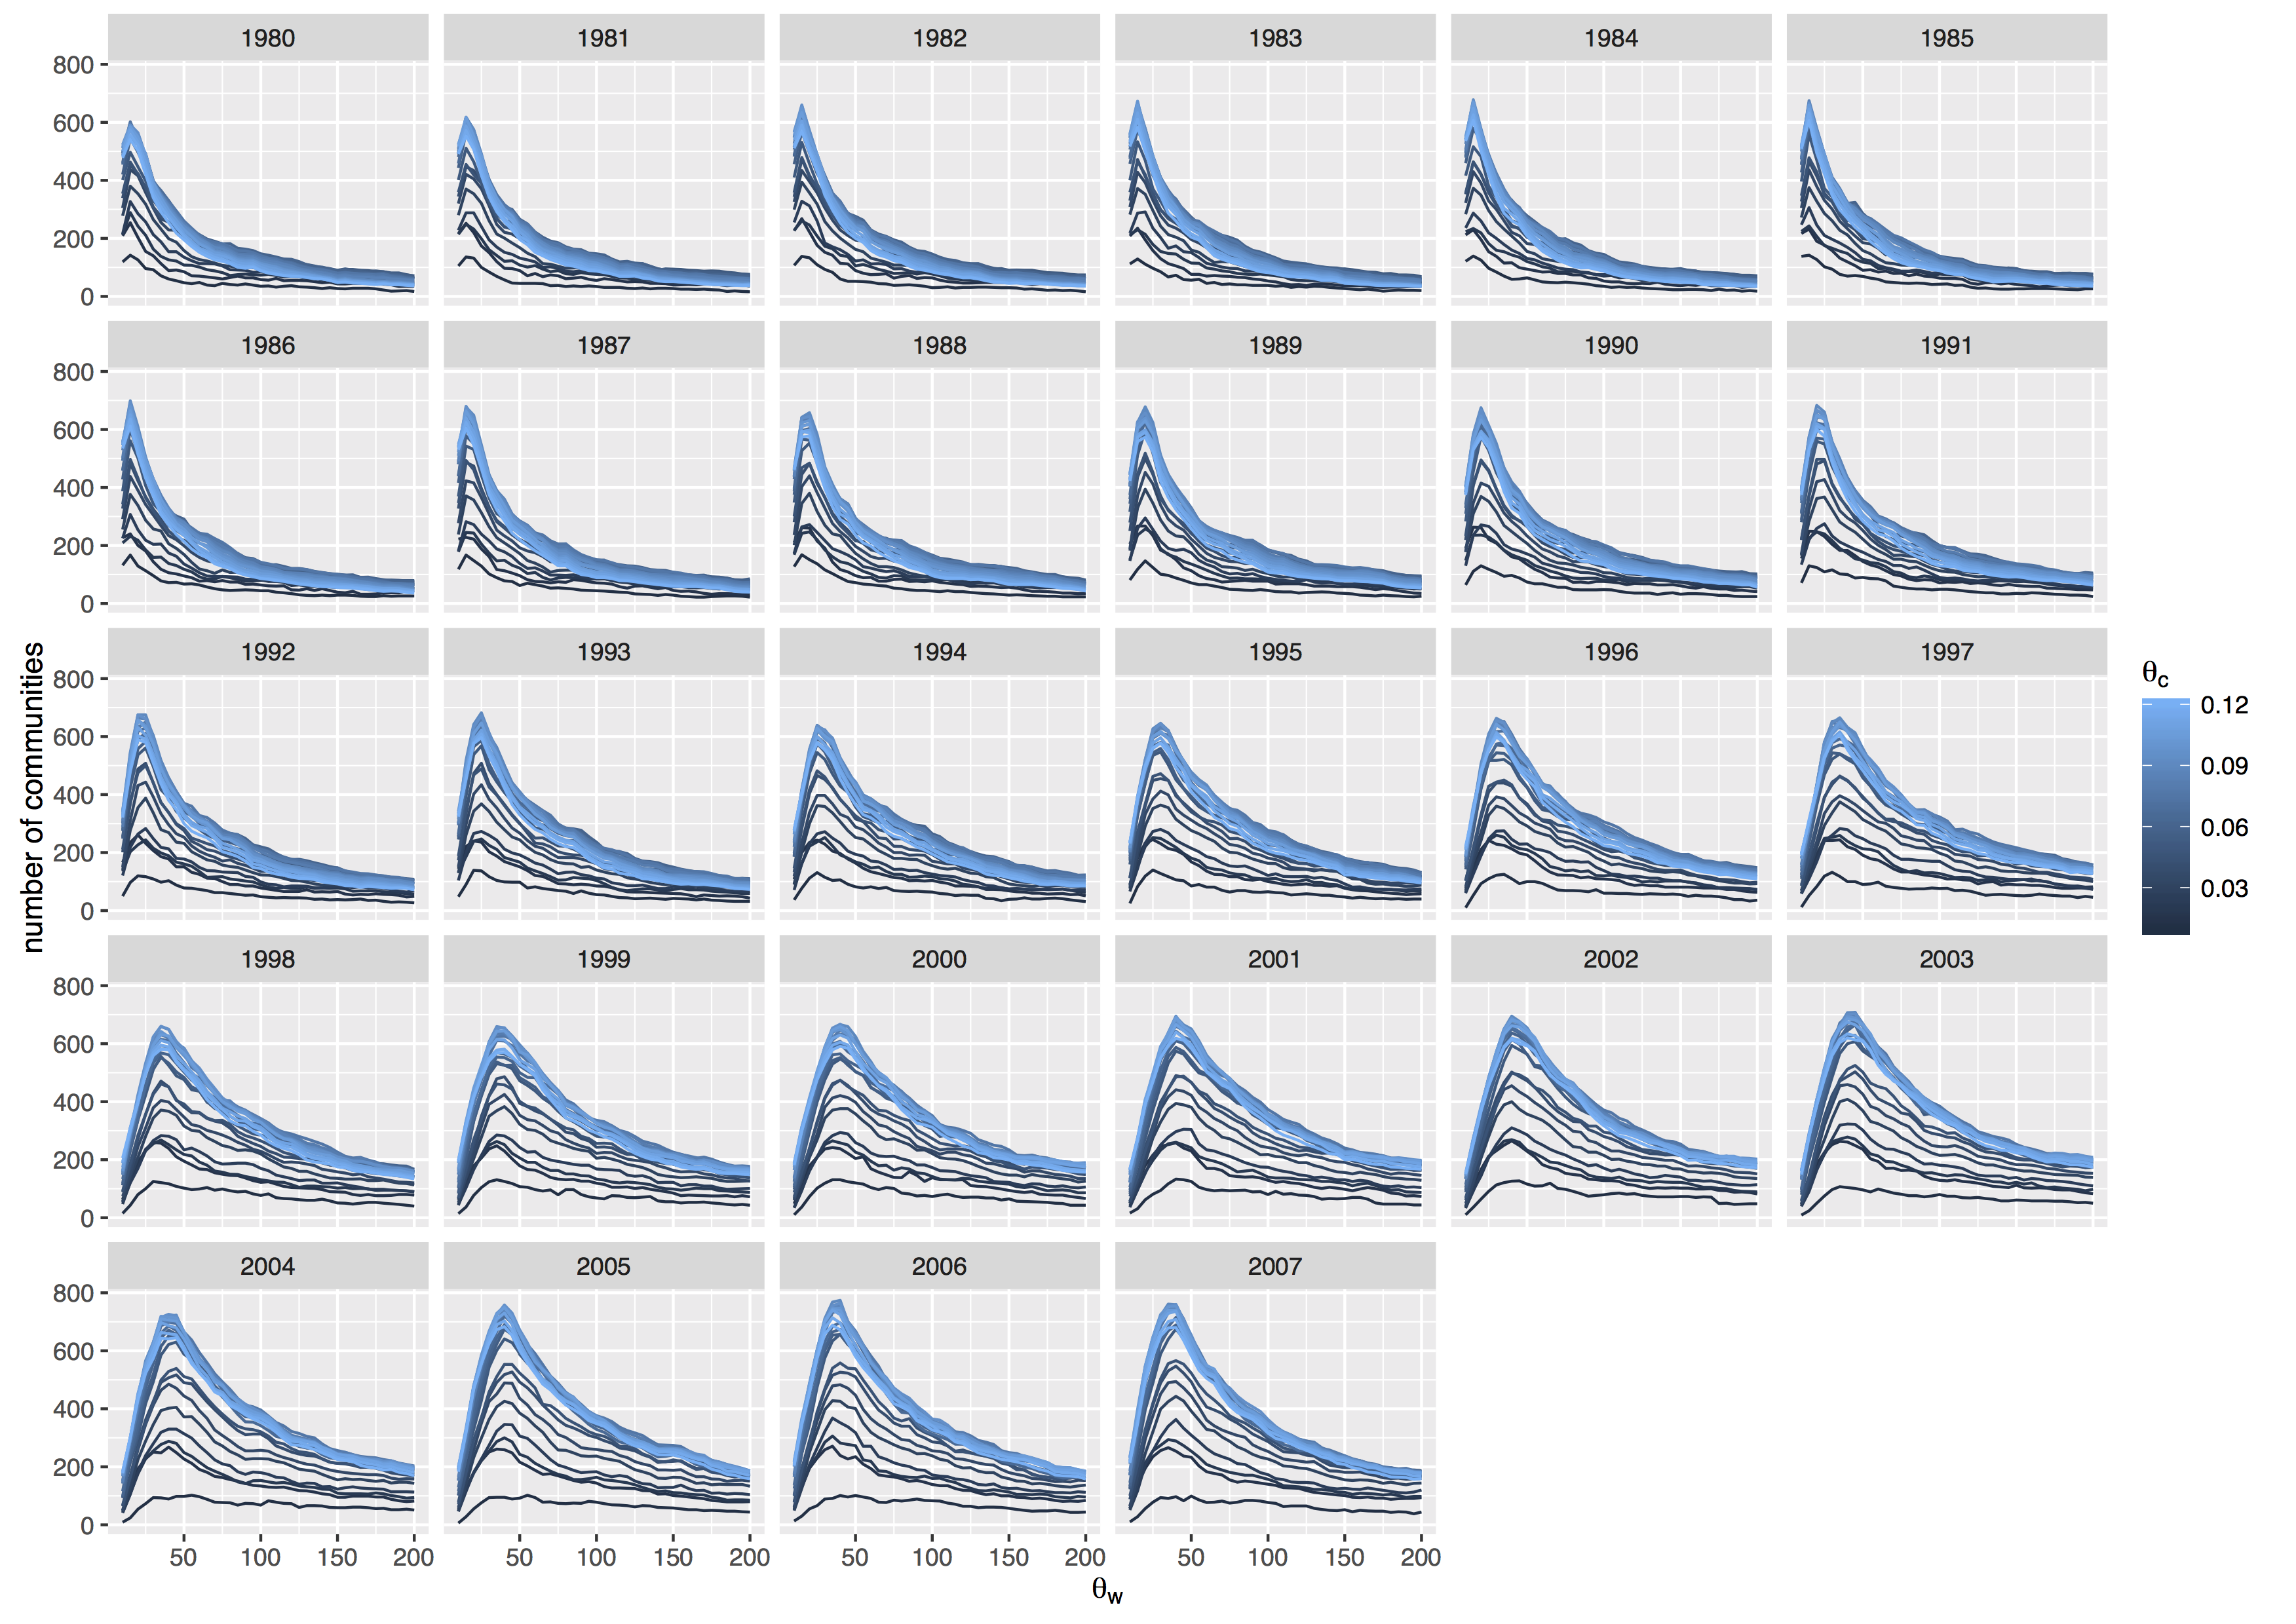
\includegraphics[width=\textheight,height=\textwidth,angle=90]{figures/commnum_thetaw_byyears.png}
\caption{Sensitivity plots for $T_0 = 4$ : Number of communities as a function of $\theta_w$, for each year.}
\label{fig:ext-sensitivity-1}
\end{figure}
%%%%%%%%%%%%%%%%%%%%

%%%%%%%%%%%%%%%%%%%%
\begin{figure}
\centering
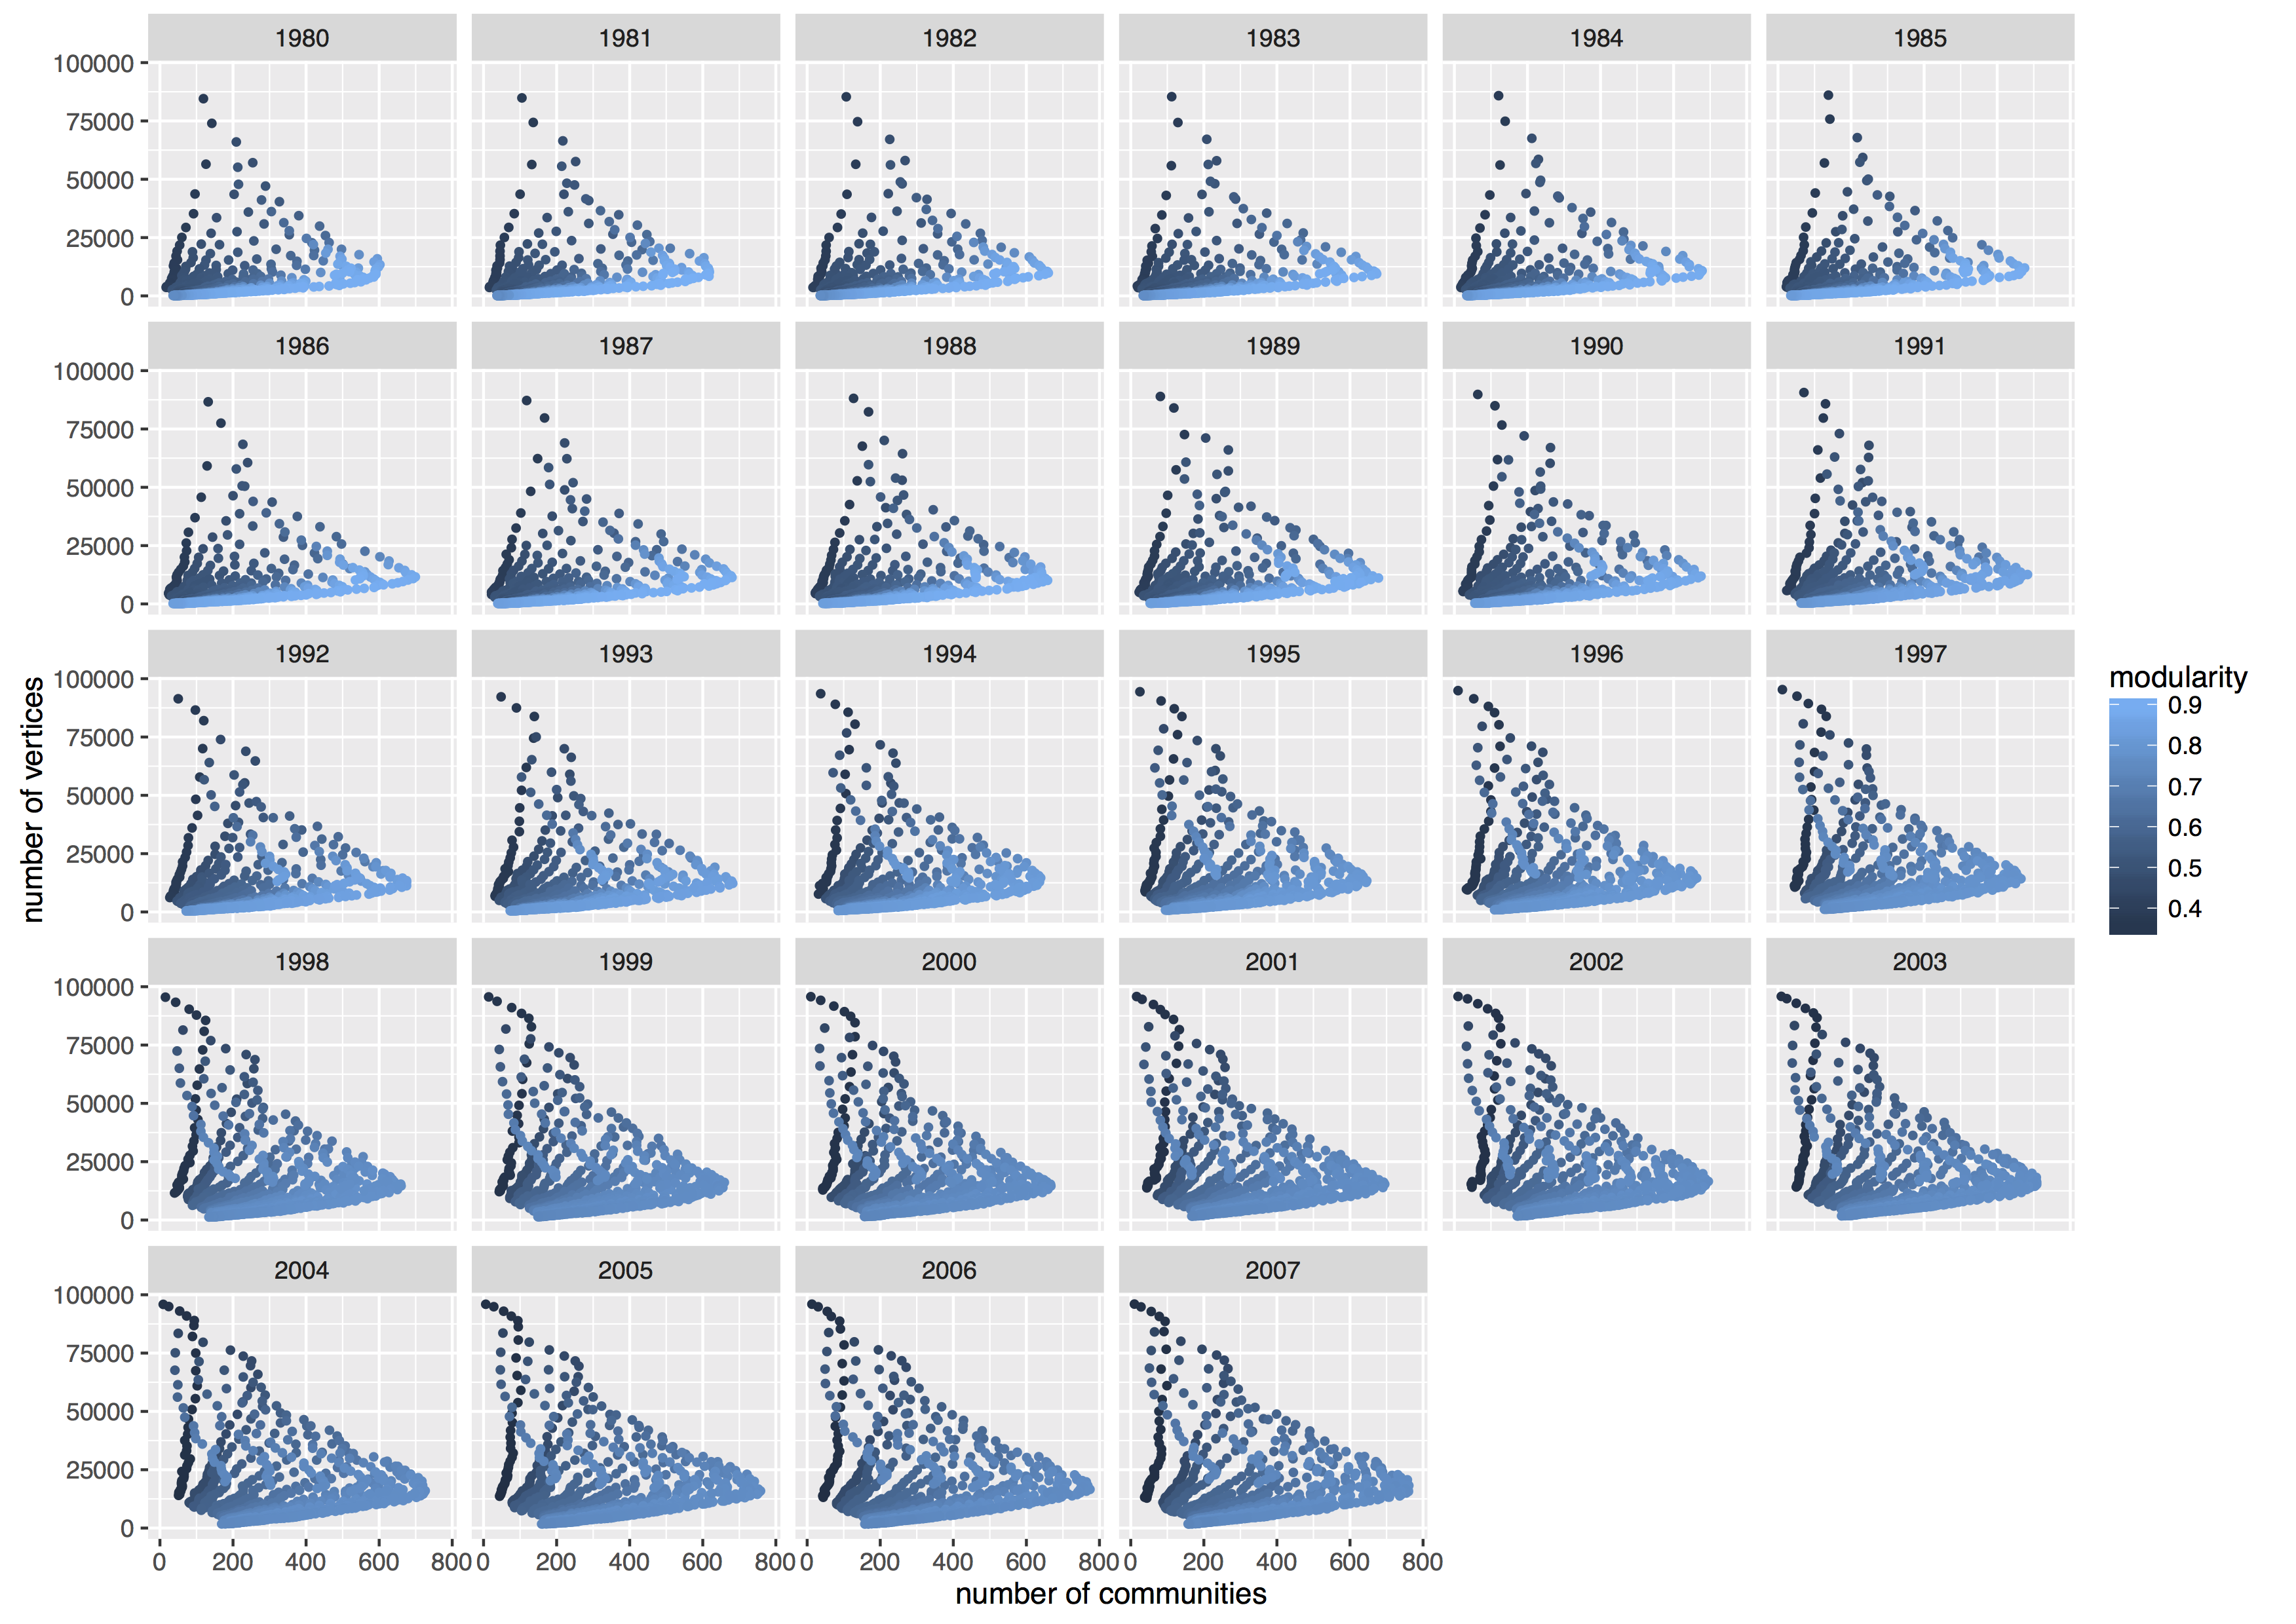
\includegraphics[width=\textheight,height=\textwidth,angle=90]{figures/vcount_comnum_pareto.png}
\caption{Sensitivity plots for $T_0 = 4$ : Pareto plots of number of communities and number of vertices, for each year.}
\label{fig:ext-sensitivity-2}
\end{figure}
%%%%%%%%%%%%%%%%%%%%

%%%%%%%%%%%%%%%%%%%%
\begin{figure}
\centering
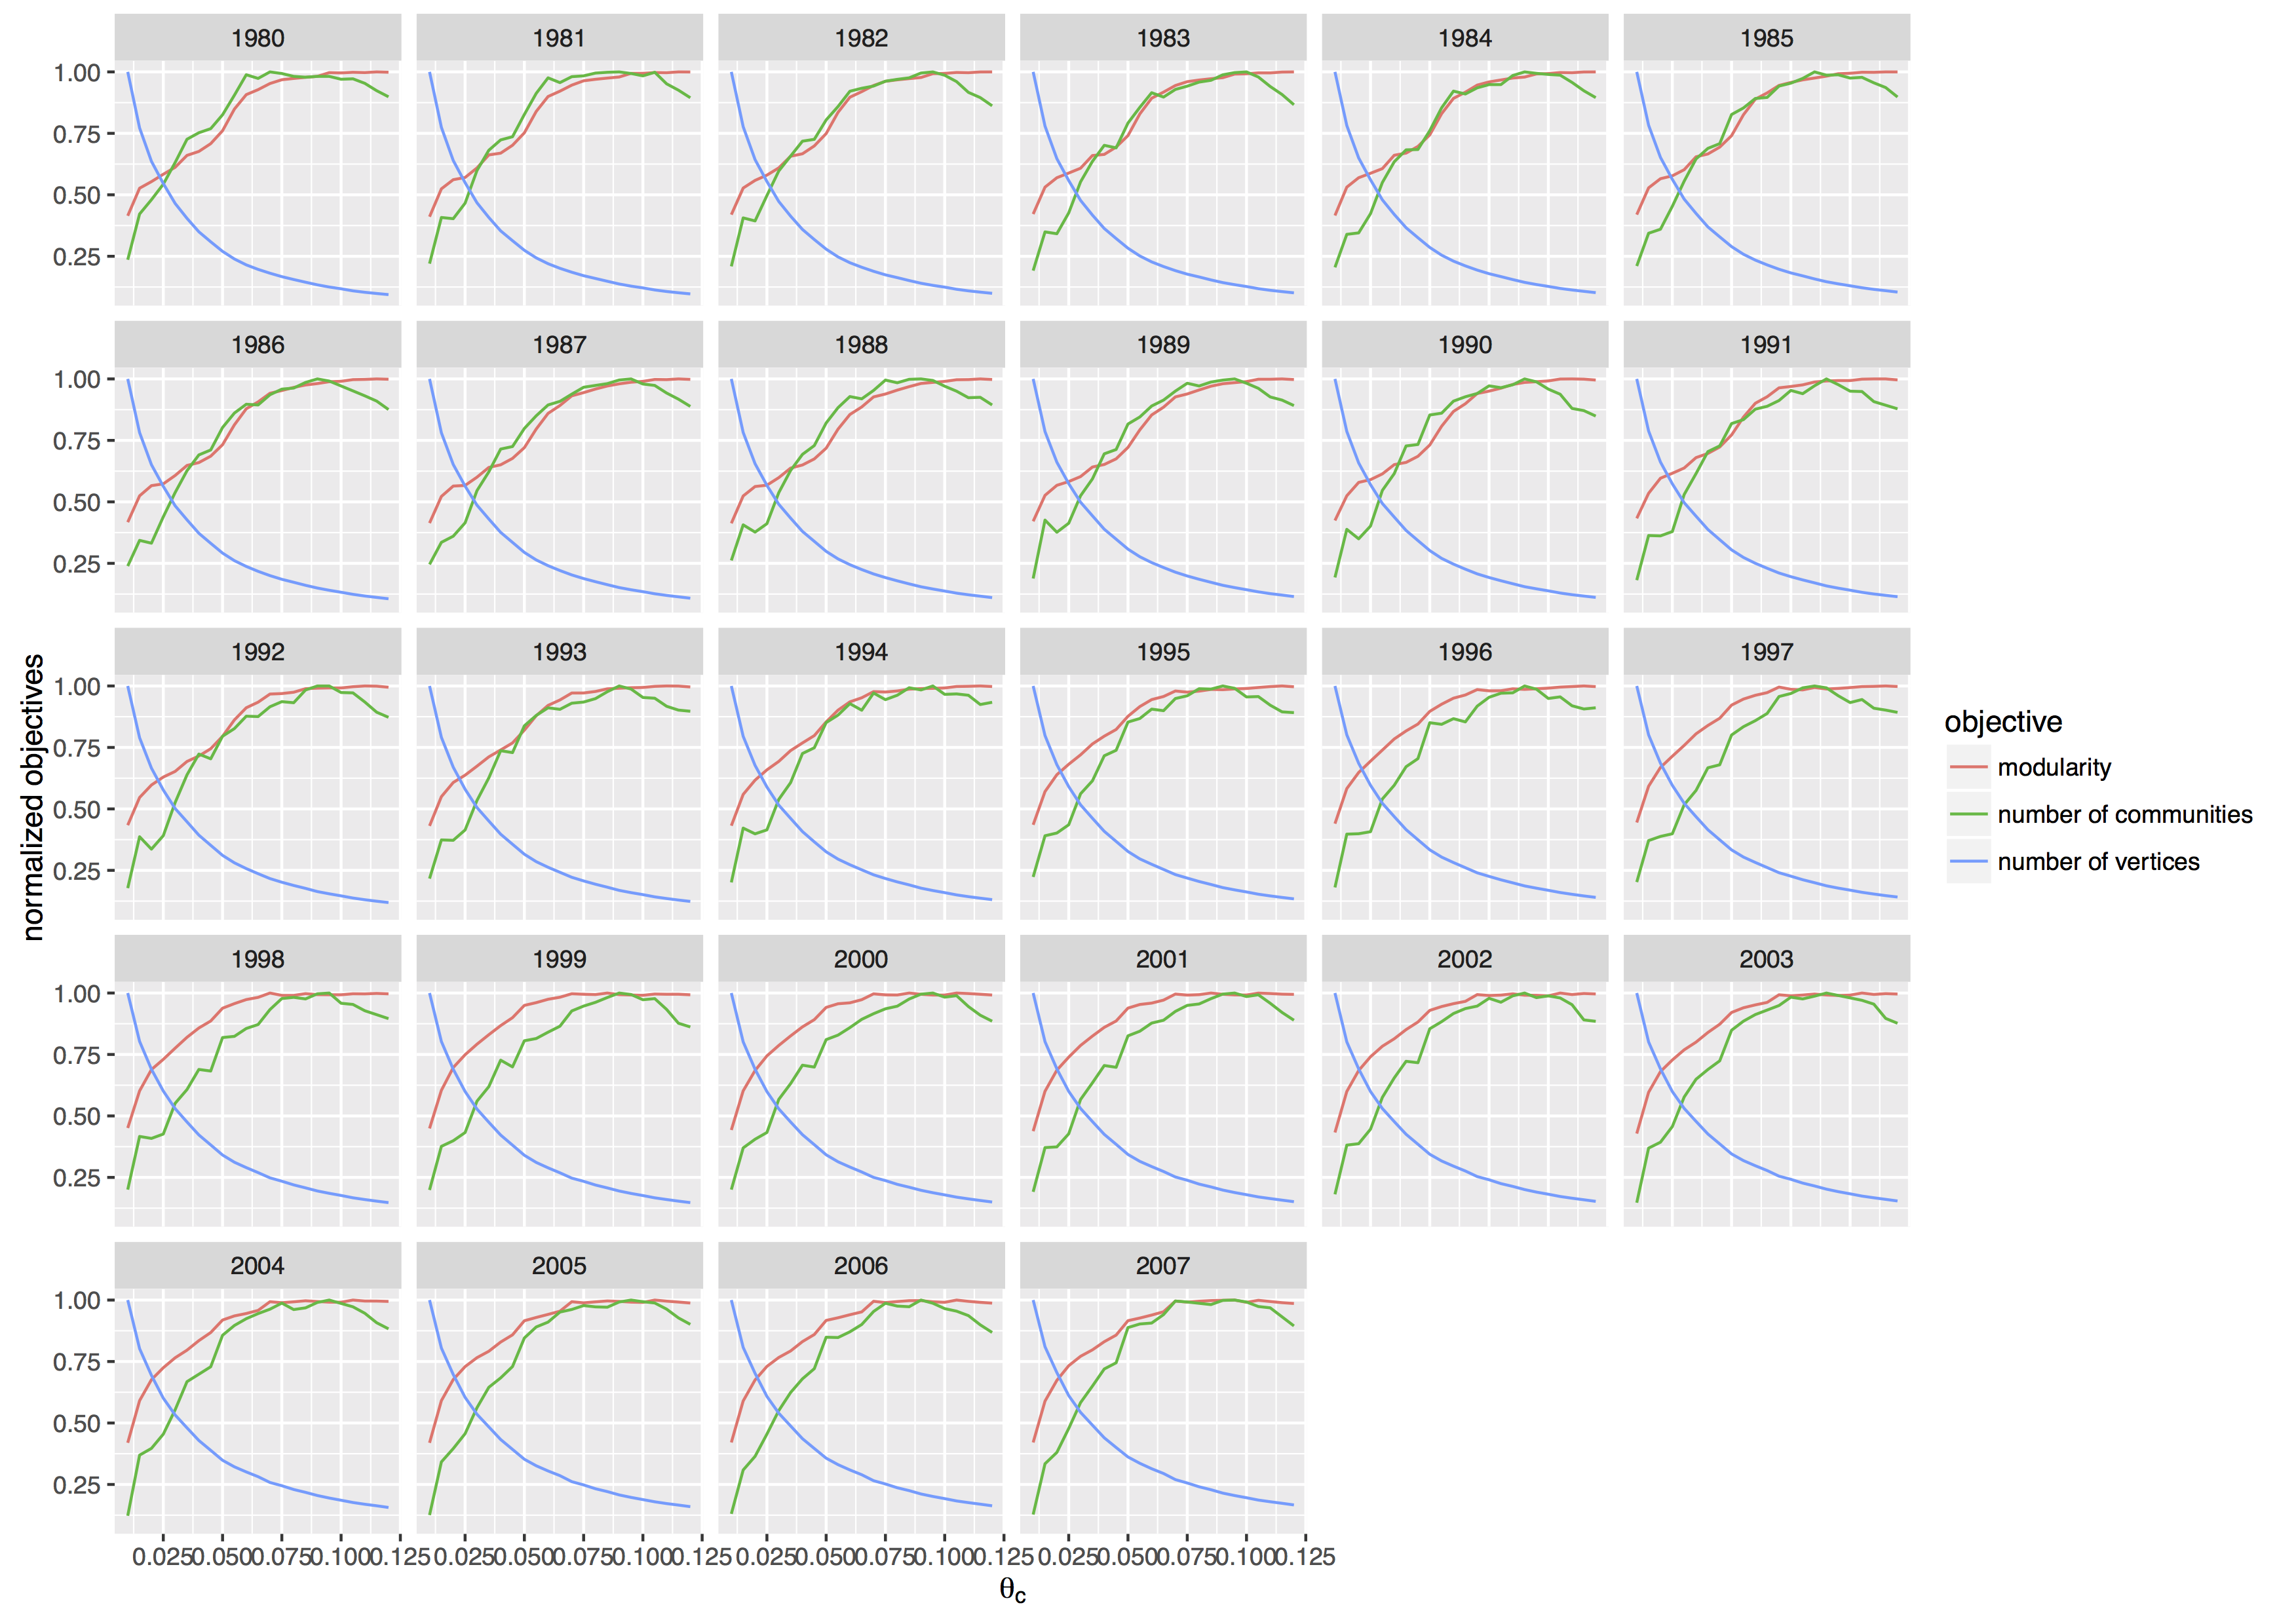
\includegraphics[width=\textheight,height=\textwidth,angle=90]{figures/normalizedObjs-dispth_eth4_1e-5.png}
\caption{Sensitivity plots for $T_0 = 4$ : normalized objective as a function of $\theta_c$, for each year.}
\label{fig:ext-sensitivity-3}
\end{figure}
%%%%%%%%%%%%%%%%%%%%



%%%%%%%%%%%%%%%%%%%%
\subsubsection*{Time-window size sensitivity}

% put some graphs for 3-years time window : same qualitative properties but a bit more noisy

We show in Fig.~\ref{fig:sensitivity-window3-1}, \ref{fig:sensitivity-window3-2} and \ref{fig:sensitivity-window3-3} the sensitivity plots used for semantic network construction optimization, for a different time window with $T_0 = 2$. The same qualitative behavior is observed (with different quantitative values, as typically $\theta_w^{(0)}$ is for example expected to vary with document number and semantic regime, thus with window size), what confirms that the method is valid across different time windows.


%%%%%%%%%%%%%%%%%%%%
\begin{figure}
\centering
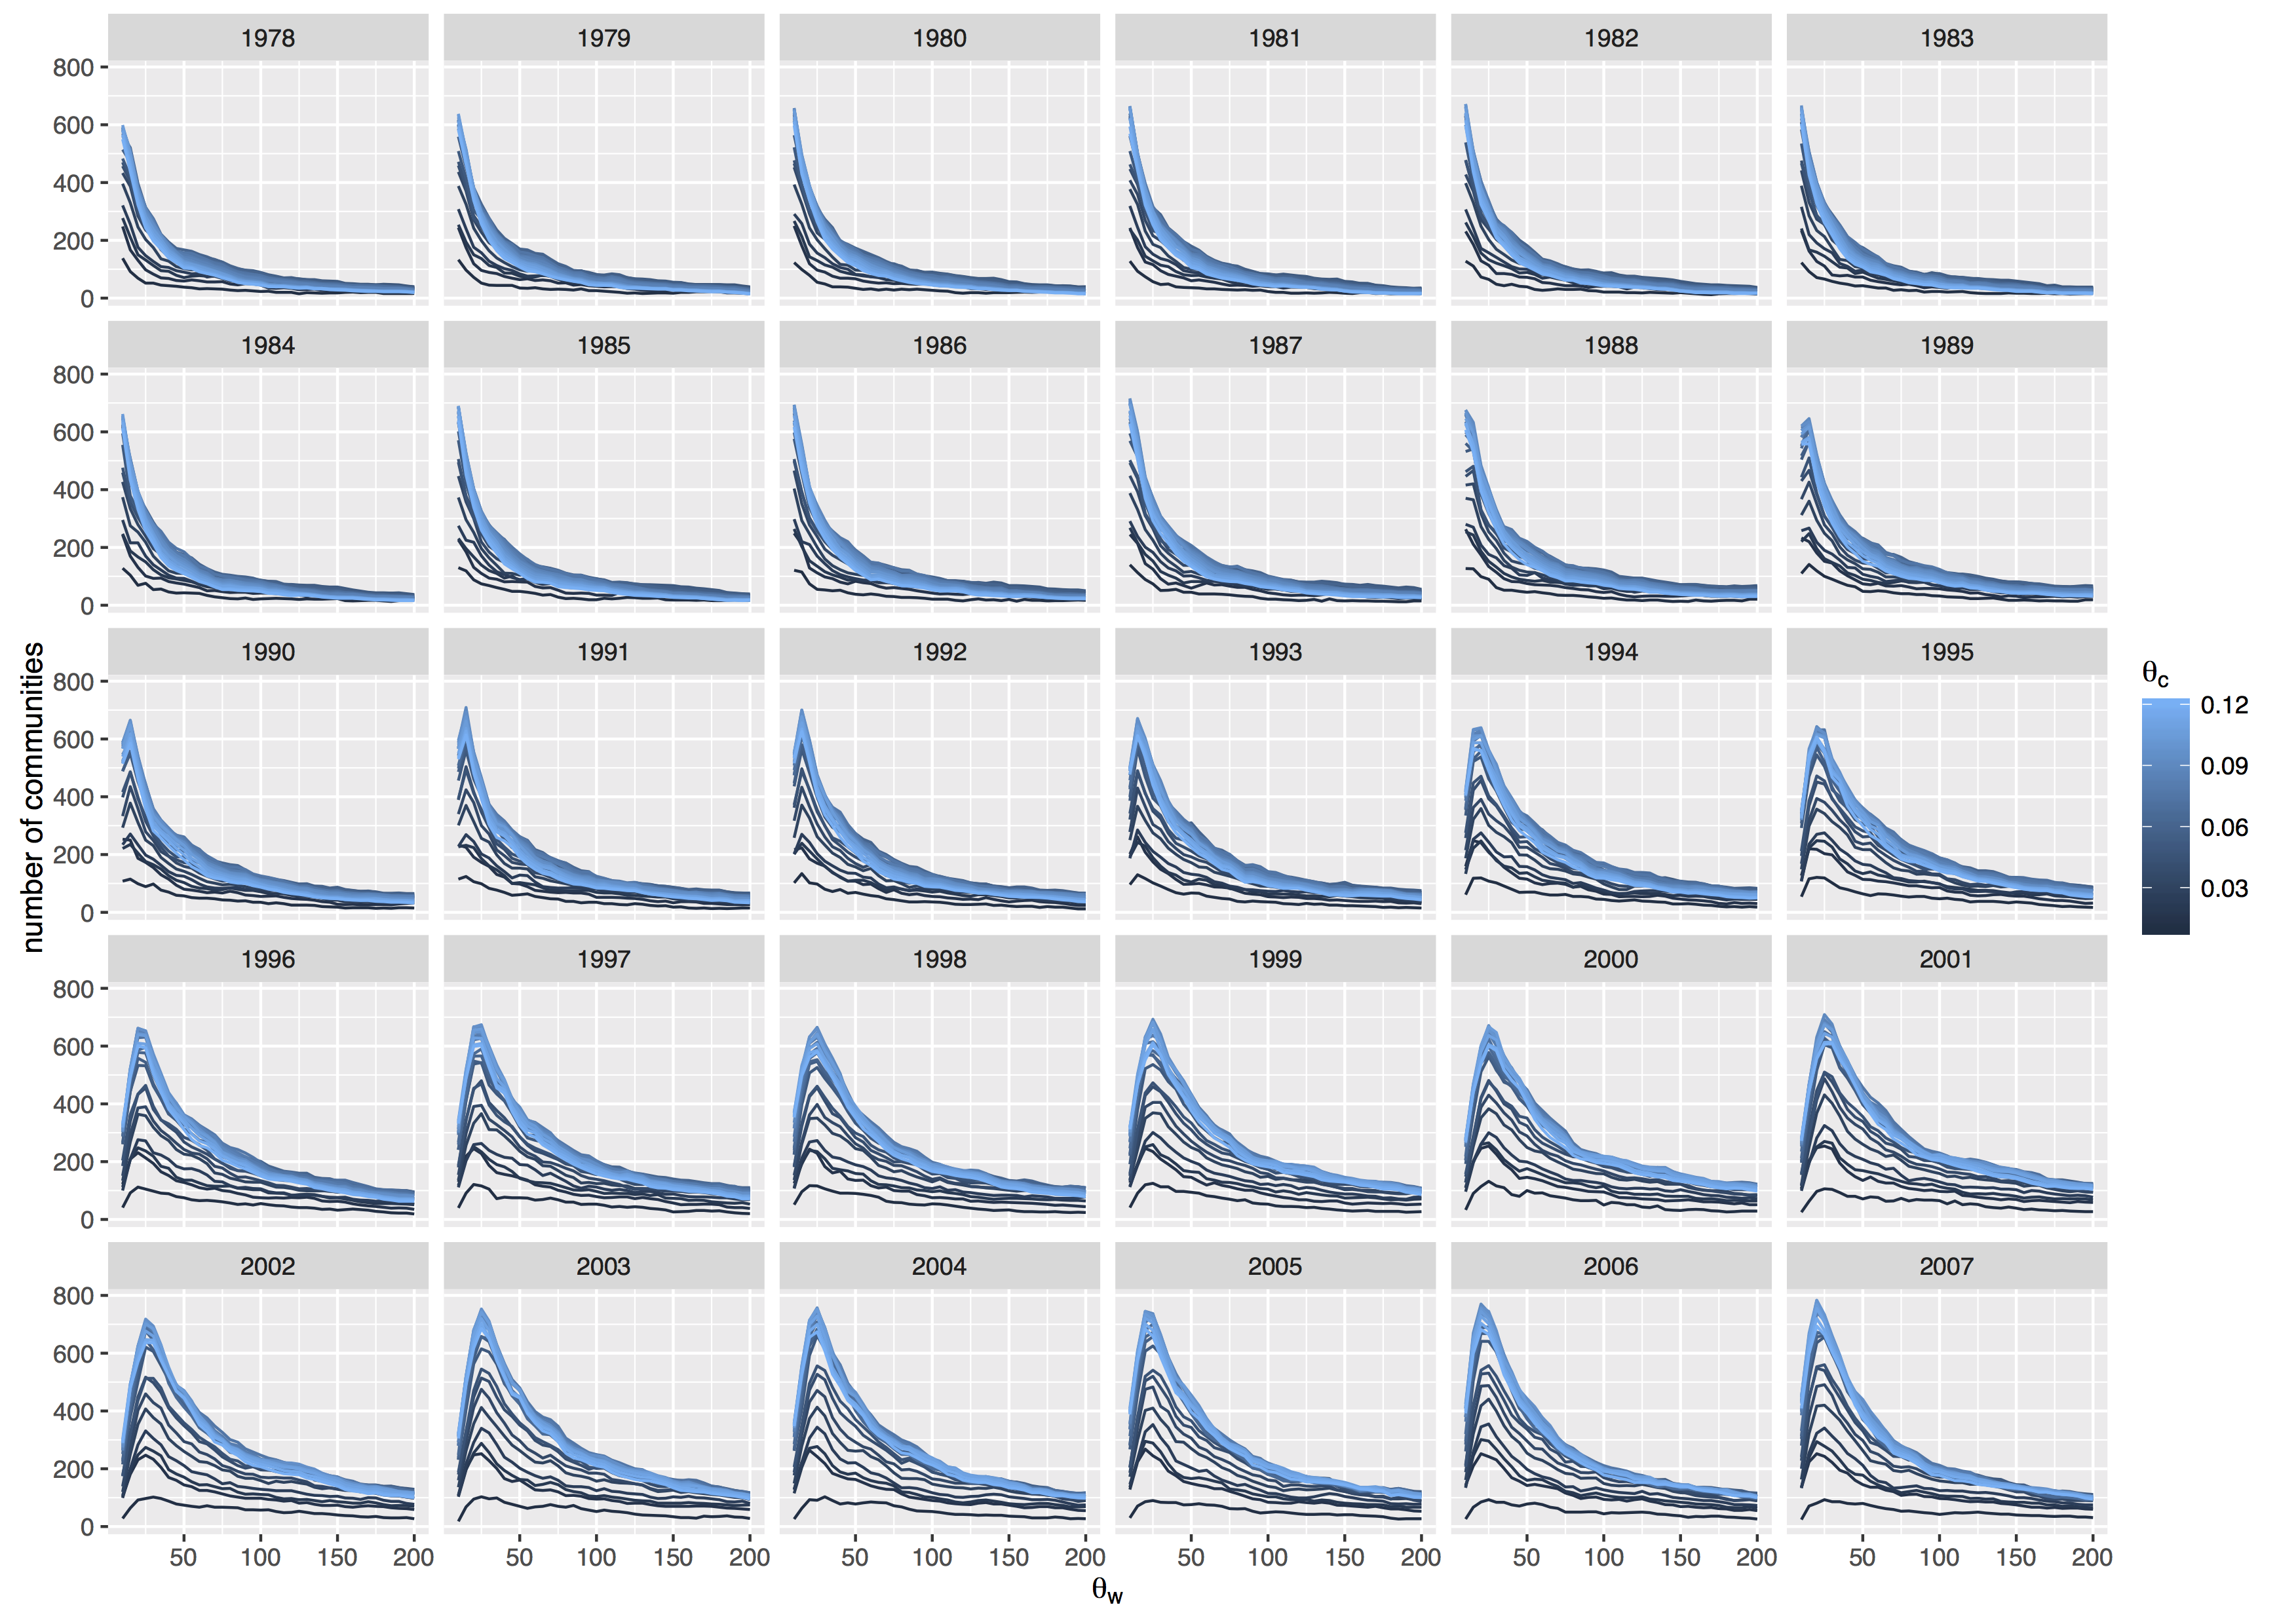
\includegraphics[width=\textheight,height=\textwidth,angle=90]{figures/commnum_thetaw_byyears_window3.png}
\caption{Sensitivity plots for $T_0 = 2$ : Number of communities as a function of $\theta_w$, for each year.}
\label{fig:sensitivity-window3-1}
\end{figure}
%%%%%%%%%%%%%%%%%%%%


%%%%%%%%%%%%%%%%%%%%
\begin{figure}
\centering
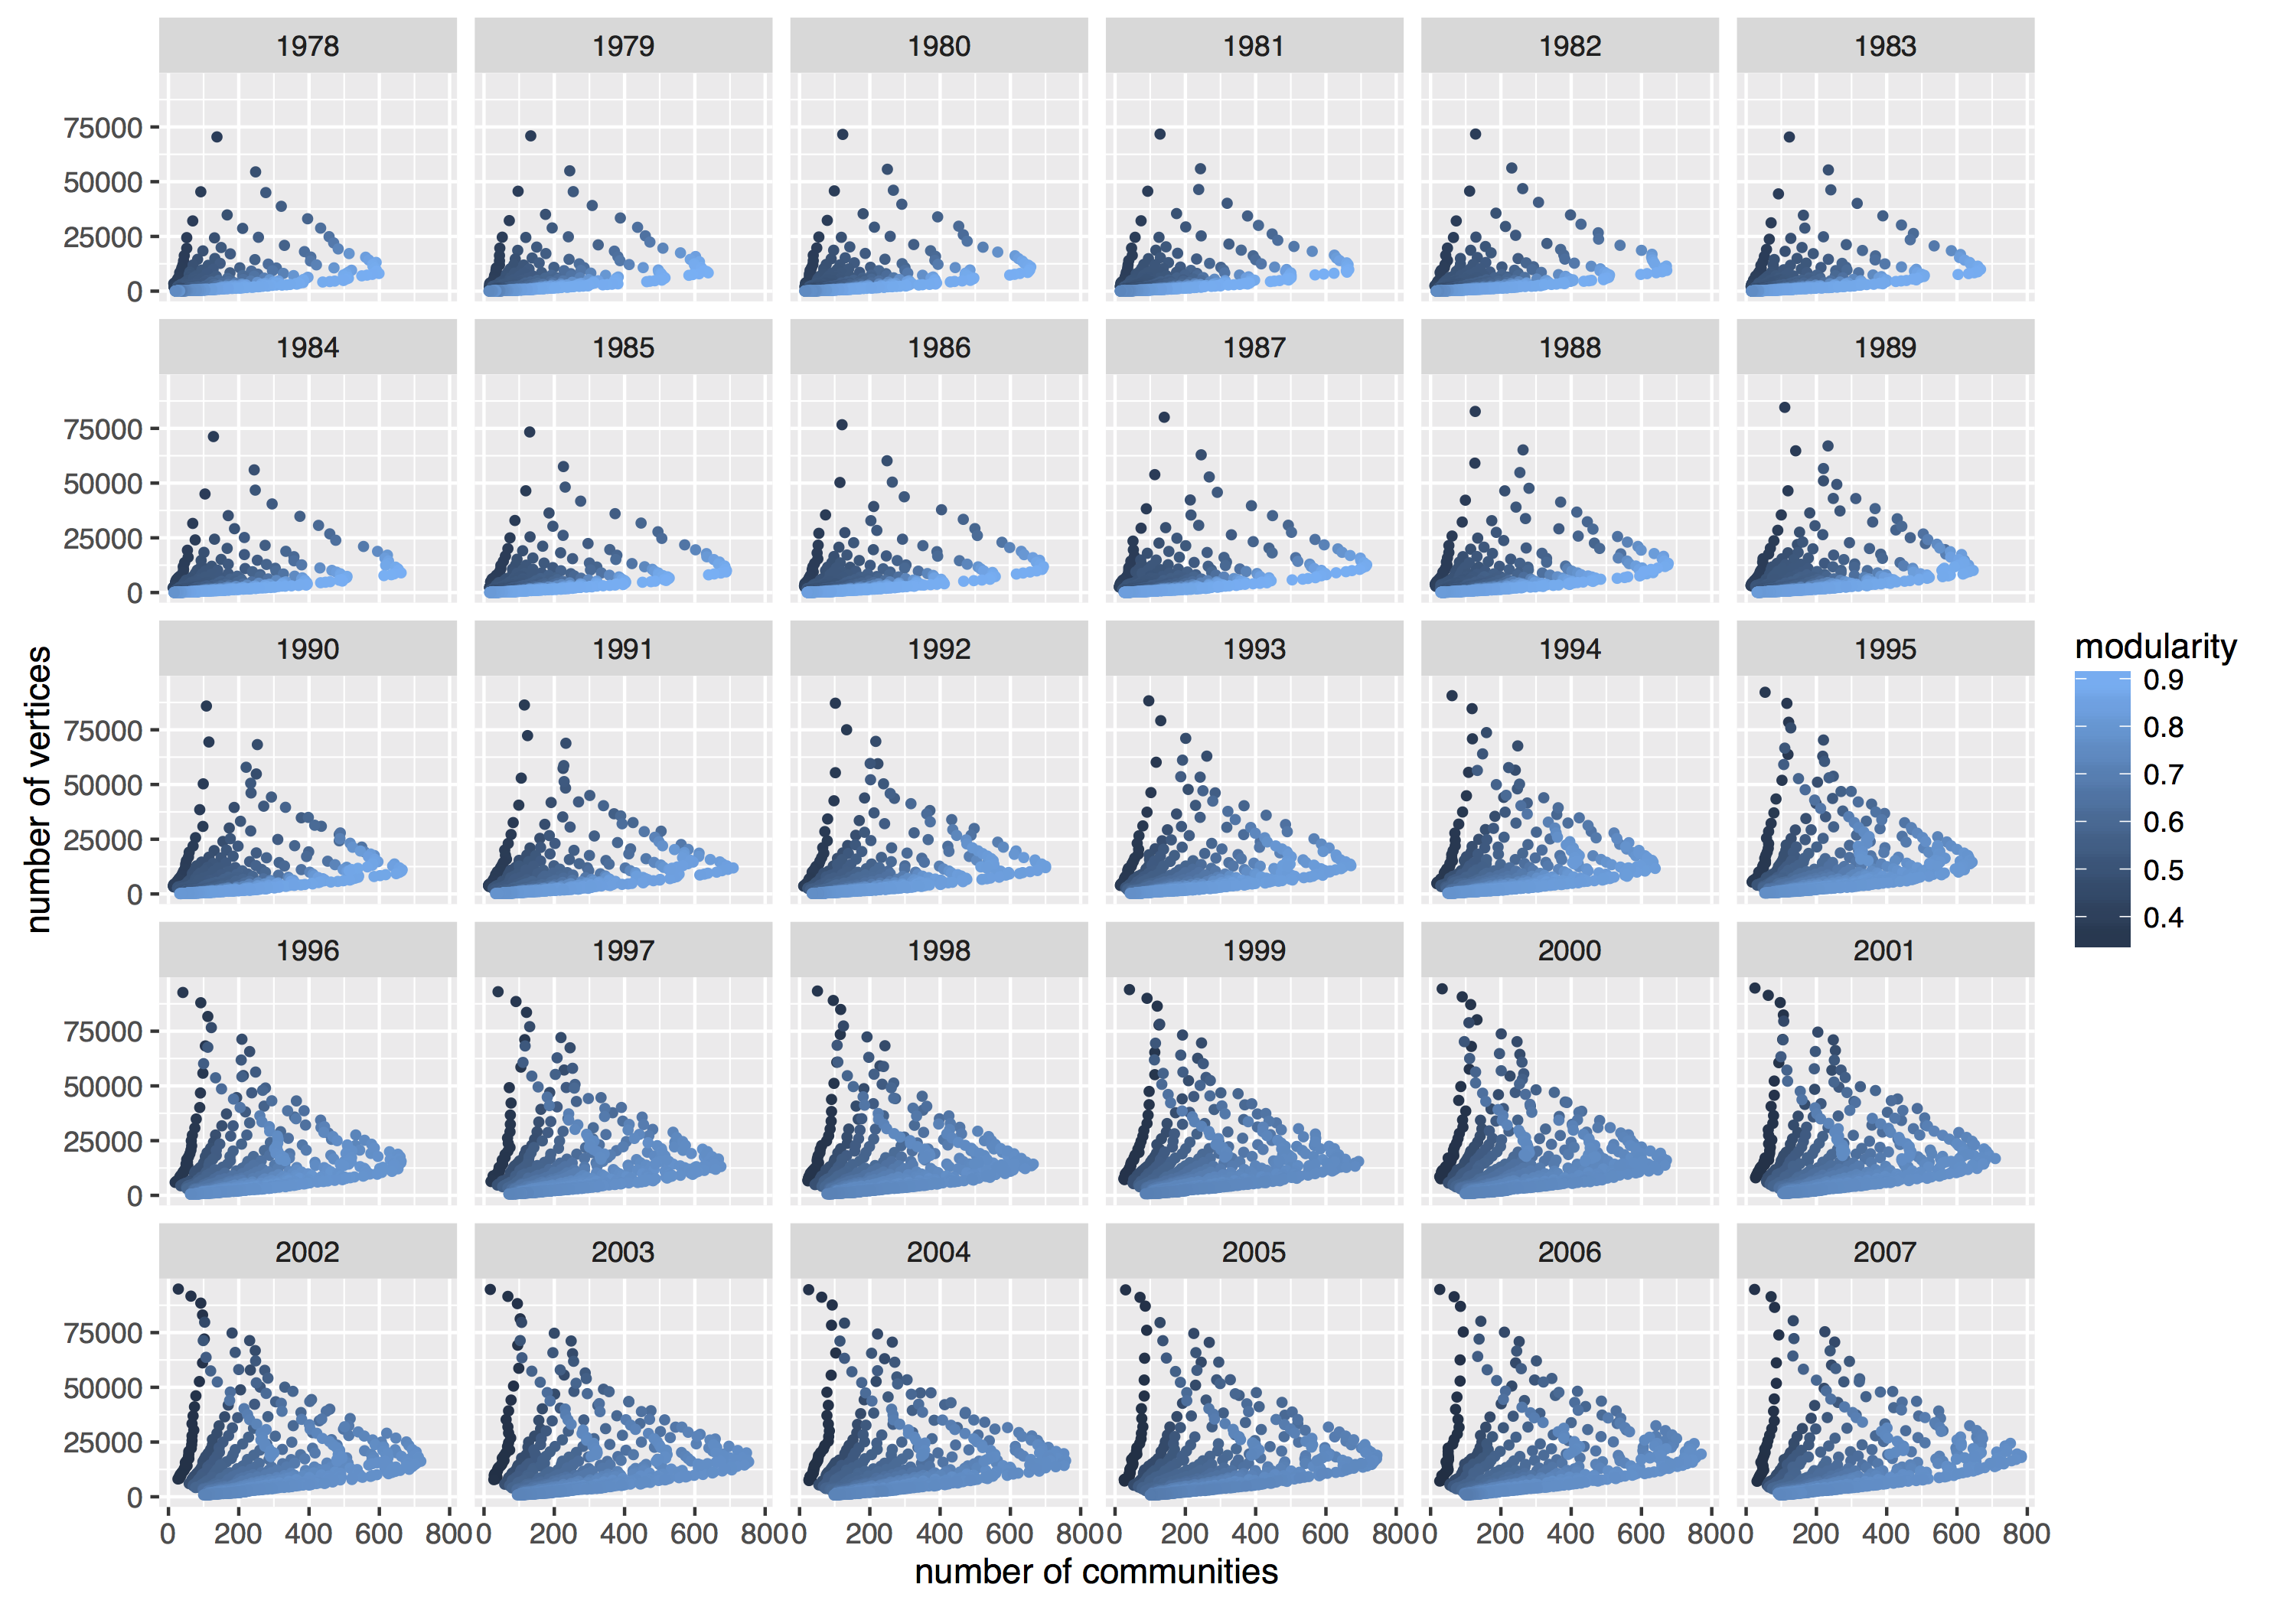
\includegraphics[width=\textheight,height=\textwidth,angle=90]{figures/vcount_comnum_pareto_window3.png}
\caption{Sensitivity plots for $T_0 = 2$ : Pareto plots of number of communities and number of vertices, for each year.}
\label{fig:sensitivity-window3-2}
\end{figure}
%%%%%%%%%%%%%%%%%%%%


%%%%%%%%%%%%%%%%%%%%
\begin{figure}
\centering
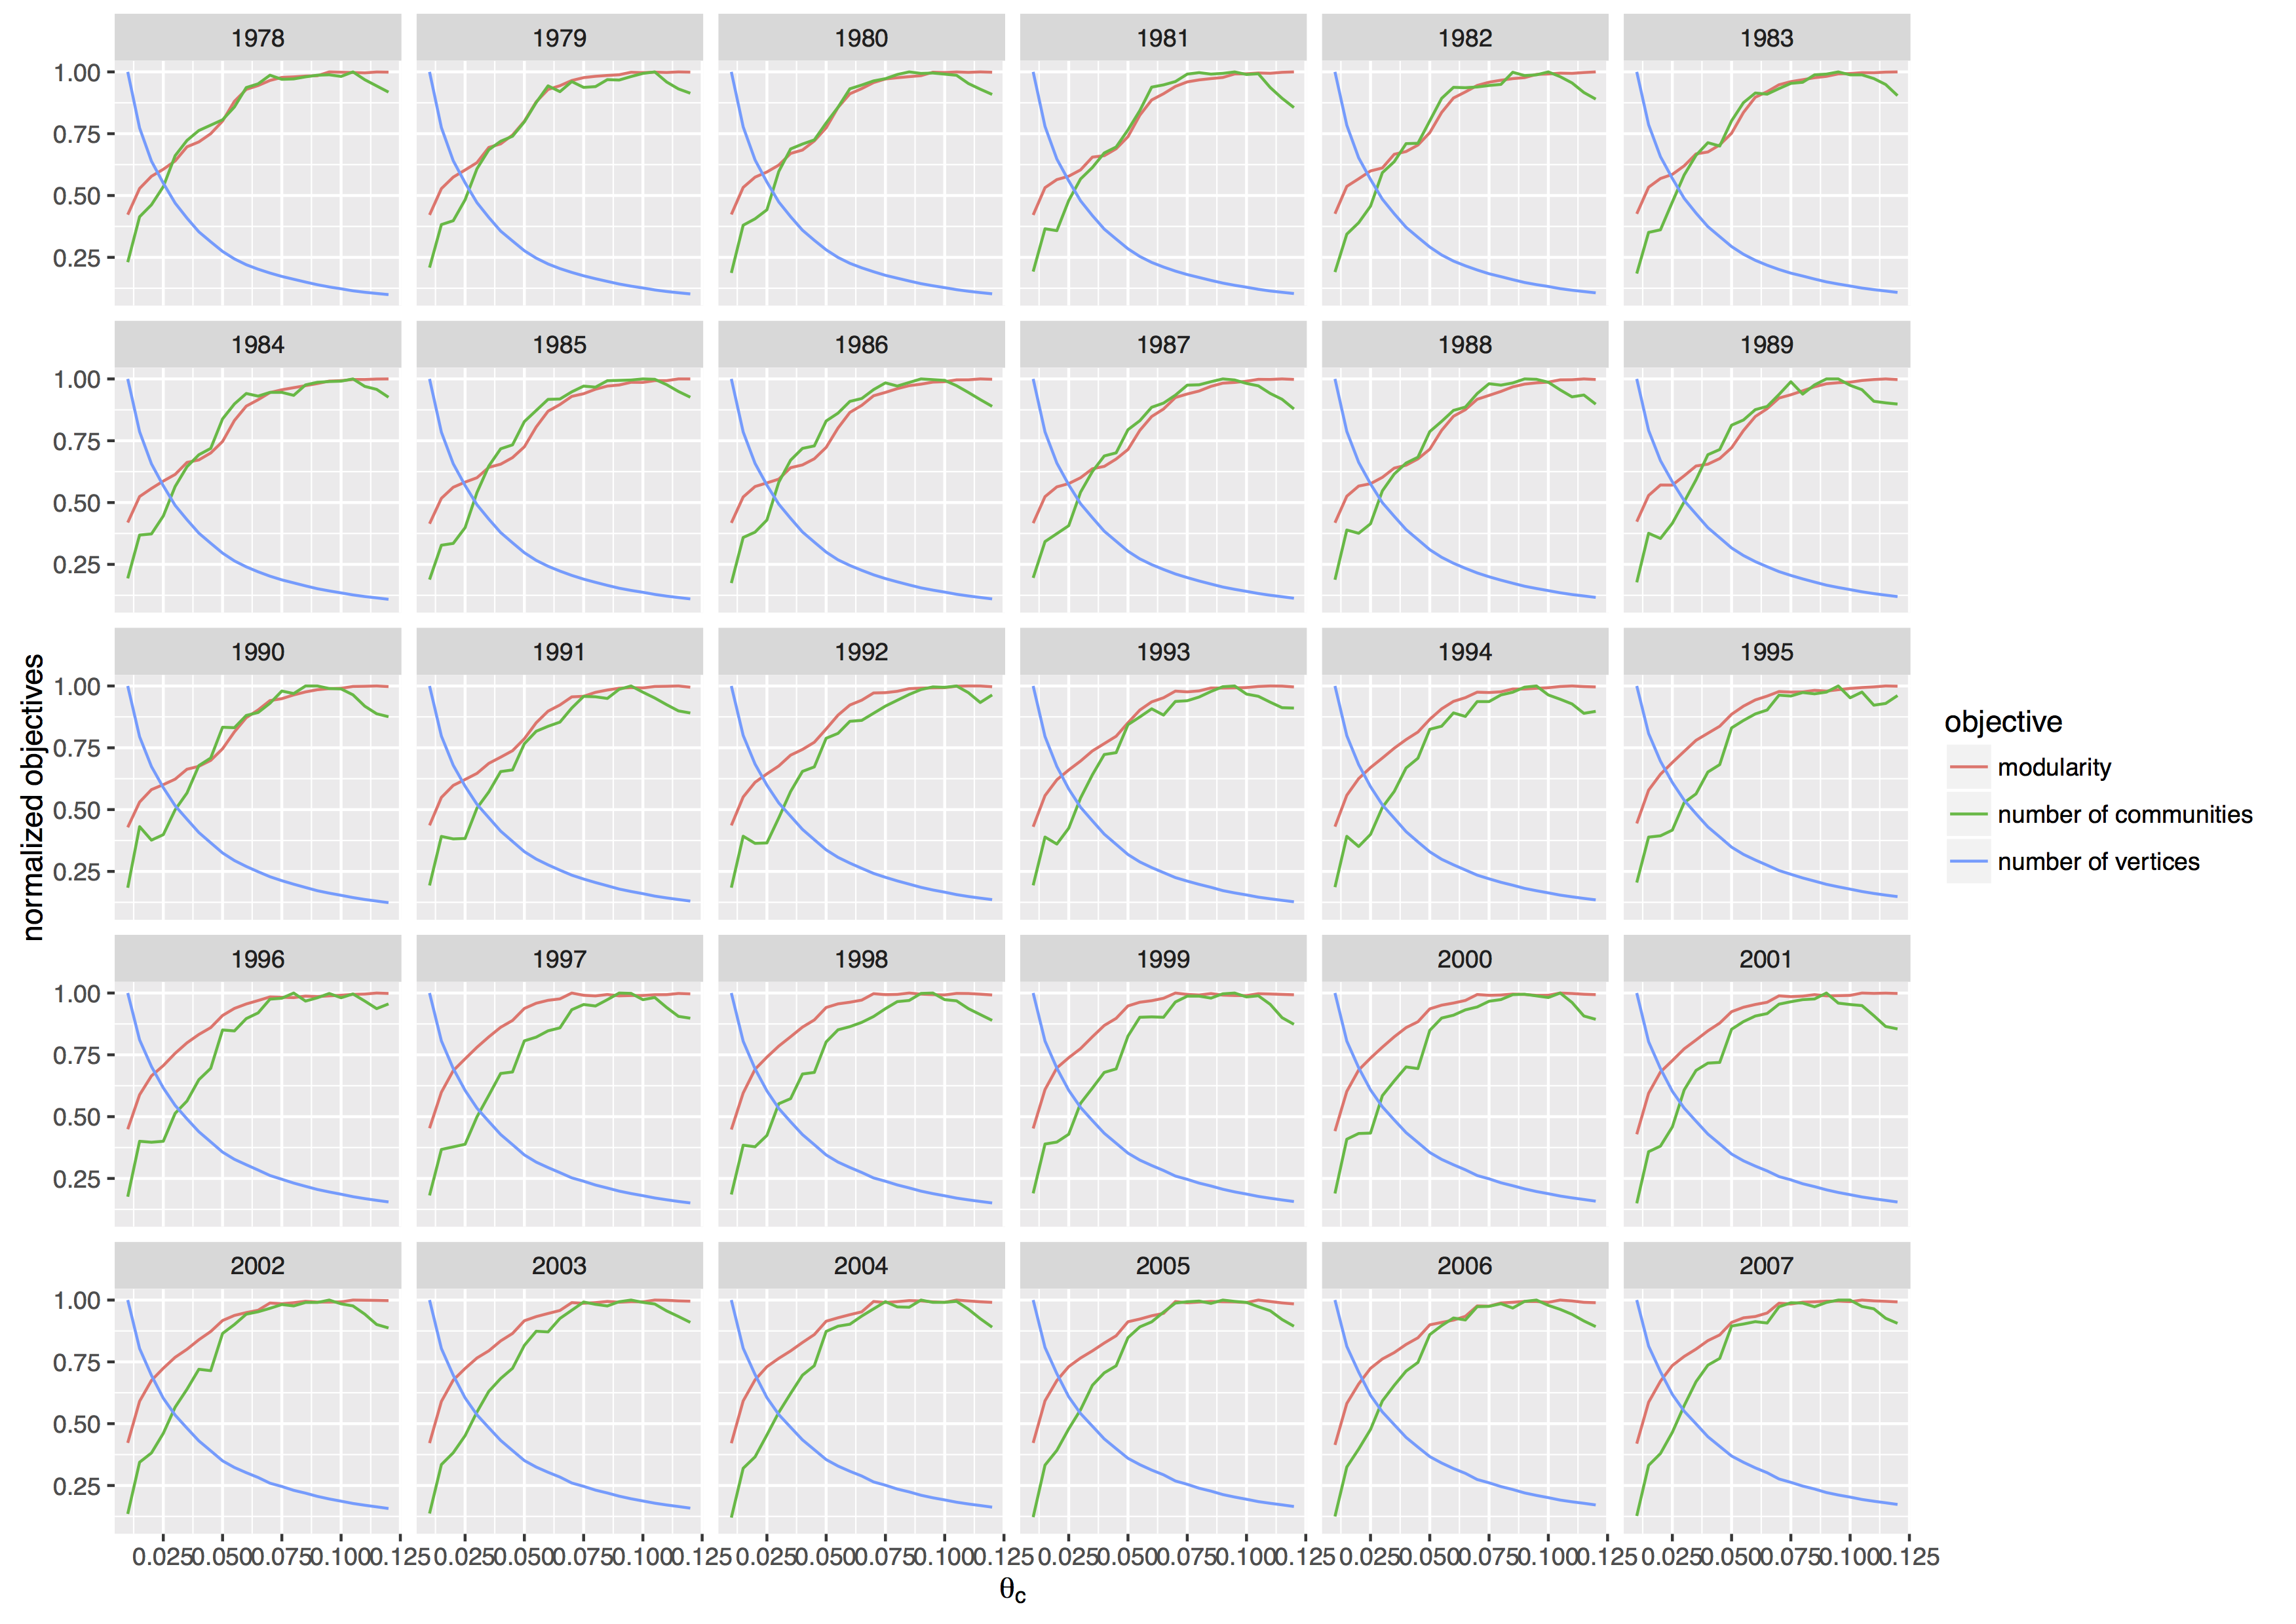
\includegraphics[width=\textheight,height=\textwidth,angle=90]{figures/normalizedObjs-dispth_window3_eth4_1e-5.png}
\caption{Sensitivity plots for $T_0 = 2$ : normalized objective as a function of $\theta_c$, for each year.}
\label{fig:sensitivity-window3-3}
\end{figure}
%%%%%%%%%%%%%%%%%%%%







%\subsubsection*{An alternative filtering method}

%Other heuristic for network construction were tested. We describe one in the following. We assume the highest degree terms do not carry specific information on particular classes and can be thus filtered given a maximal degree threshold $k{max}$. Similarly, edge with small weight must not carry significant information and are filtered according to a minimal edge weight threshold $w_{min}$. Keywords are preliminary filtered by a document frequency window $\left[ f_{min},f_{max} \right]$ which is slightly different from network filtering and complementary. A sensitivity analysis of resulting network topology to these parameters is shown in Fig. .

%
%%%%%%%%%%%%%%%%%%%%%
%\begin{figure}[!ht]
%% values of some topological measures in 2D parameter space
%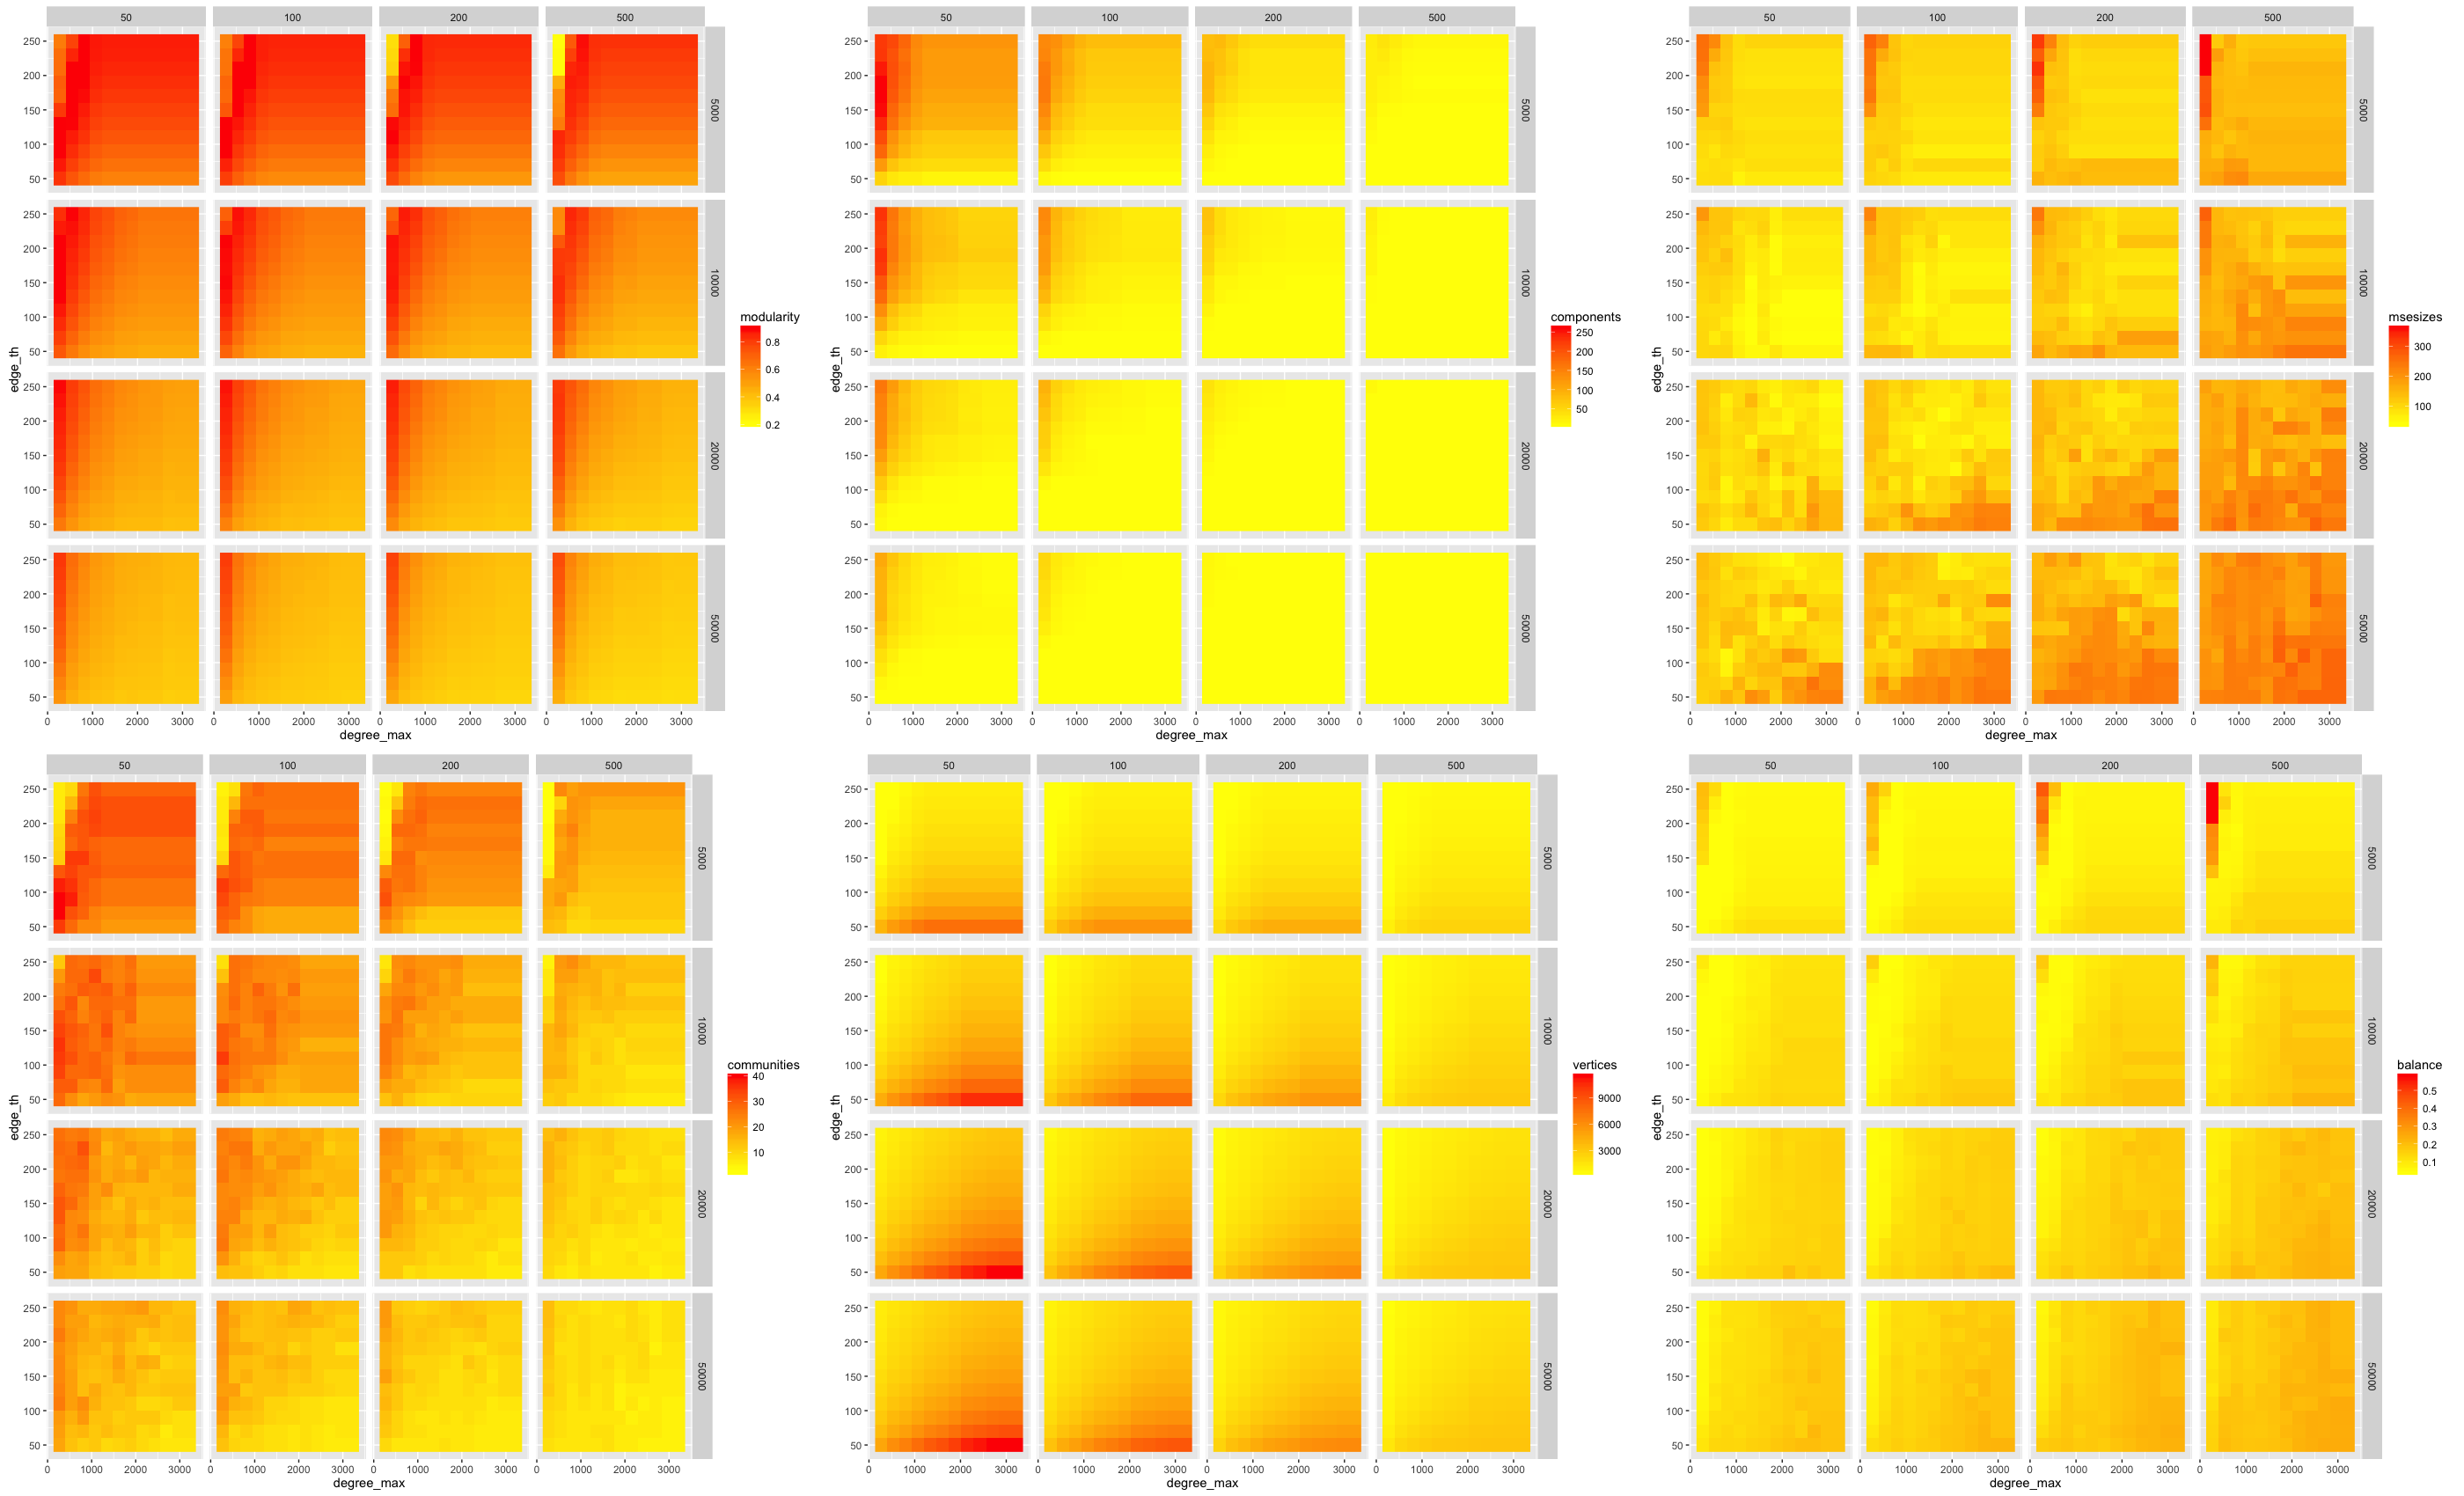
\includegraphics[width=\textwidth]{figures/graph_sens_2010_msesizes}
%\caption{Variation of semantic network indicators across a 4-dimensional parameter space (figure-level axis : $(k_{max},w_{min})$; meta axis: $(f_{min},f_{max})$), for year 2010, where indicators are modularity (louvain method), number of connected components, proximity of class size distribution to technological classes size distribution, communities number, network size, community size balance. A good optimization compromise is given here by $()$.}
%% TODO change with proportion parameters in new figure
%% TODO detail which obj to be minimized etc in supplementary material
%\end{figure}
%%%%%%%%%%%%%%%%%%%%%
%



\end{document}
